\documentclass[12pt]{article}
\usepackage[a4paper, top=2.5cm, bottom=2.5cm, left=1.5cm, right=1.5cm]{geometry}
\usepackage{amsmath, amsfonts, amssymb, mathtools}
\usepackage{fancyhdr, setspace, parskip}
\usepackage{graphicx, caption, subfig, array, multirow}
\usepackage{hyperref, enumitem, cancel}
\usepackage[T1]{fontenc}
\usepackage{tgtermes}
\usepackage[dvipsnames]{xcolor}
\usepackage{tocloft}
\usepackage{titlesec}
\usepackage{lipsum}  

\definecolor{DarkBlue}{RGB}{10, 0, 80}

% Hyperlink setup
\hypersetup{
    colorlinks=true,
    linkcolor=DarkBlue,
    filecolor=BrickRed,      
    urlcolor=RoyalBlue,
}


% Header and footer customization
\fancyhead{}
\fancyhead[L]{
{\fontfamily{lmss}{\color{DarkBlue}
\textbf{\leftmark}
}}
}
\fancyhead[R]{
{\fontfamily{ppl}\selectfont {\color{DarkBlue}
{Deep RL Course [Spring 2025]}
}}
}

\fancyfoot{}
\fancyfoot[C]{
{\fontfamily{lmss}{\color{BrickRed}
\textbf{\thepage}
}}
}

\renewcommand{\sectionmark}[1]{ \markboth{\thesection\quad #1}{} }

\renewcommand{\headrule}{{\color{BrickRed}\hrule width\headwidth height 0.5pt}}
\renewcommand{\footrulewidth}{0pt}


% Table of Contents customizations
\renewcommand{\cftsecafterpnum}{\vskip6pt}
\renewcommand{\cftsubsecafterpnum}{\vskip3pt}
\renewcommand{\cftsubsubsecafterpnum}{\vskip3pt}
\renewcommand{\cftsecfont}{\sffamily\large}
\renewcommand{\cftsubsecfont}{\sffamily}
\renewcommand{\cftsubsubsecfont}{\sffamily}
% \renewcommand{\cftsecdotsep}{1}
\renewcommand{\cftsubsecdotsep}{1}
\renewcommand{\cftsubsubsecdotsep}{1}


% Section title styles
\titleformat*{\section}{\LARGE\bfseries\color{DarkBlue}}
\titleformat*{\subsection}{\Large\bfseries\color{DarkBlue}}
\titleformat*{\subsubsection}{\large\bfseries\color{DarkBlue}}

\definecolor{light-gray}{gray}{0.95}
\newcommand{\code}[1]{\colorbox{light-gray}{\texttt{#1}}}

% Start of the document
\pagestyle{fancy}

%%%%%%%%%%%%%%%%%%%%%%%%%%%%%%%%%%%%%%%%%%%%%%%%%

\begin{document}

\pagenumbering{gobble}
\thispagestyle{plain}

\begin{center}

\vspace*{-1.5cm}
\begin{figure}[!h]
    \centering
    
\includegraphics[width=0.7\linewidth]{figs/cover-std.png}
\end{figure}

{
\fontfamily{ppl}

{\color{DarkBlue} {\fontsize{30}{50} \textbf{
Deep Reinforcement Learning
}}}

{\color{DarkBlue} {\Large
Professor Mohammad Hossein Rohban
}}
}


\vspace{20pt}

{
\fontfamily{lmss}

{\color{RedOrange}
{\Large
Solution for Homework 13:
}\\
}
{\color{BrickRed}
\rule{12cm}{0.5pt}

{\Huge
Multi-Agent RL

}
\rule{12cm}{0.5pt}
}

\vspace{10pt}

{\color{RoyalPurple} { \small By:} } \\
\vspace{10pt}

{\color{Blue} { \LARGE [Full Name] } } \\
\vspace{5pt}
{\color{RoyalBlue} { \Large [Student Number] } }


\vspace*{\fill}
\begin{center}
\begin{tabular}{ccc}
    
\includegraphics[width=0.14\linewidth]{figs/sharif-logo.png} & 
\includegraphics[width=0.14\linewidth]{figs/riml-logo.png} & 
\includegraphics[width=0.14\linewidth]{figs/dlr-logo.png} \\
\end{tabular}
\end{center}


\vspace*{-.25cm}

{\color{YellowOrange} {
\rule{10cm}{0.5pt} \\
\vspace{2pt}
\large Spring 2025}
}}
\vspace*{-1cm}

\end{center}

%%%%%%%%%%%%%%%%%%%%%%%%%%%%%%%%%%%%%%%%%%%%%%%%%

\newpage
\pagenumbering{gobble}

{\fontfamily{lmss}\selectfont {\color{DarkBlue}

\subsection*{Grading}

The grading will be based on the following criteria, with a total of 110 points:

\[
\begin{array}{|l|l|}
\hline
\textbf{Task} & \textbf{Points} \\
\hline
\text{Task 1} & 50 \\
\text{Task 2} & 50 \\

\hline
\text{Clarity and Quality of Code} & 5 \\
\text{Clarity and Quality of Report} & 5 \\
\hline
\text{Bonus 1} & 5 \\
\text{Bonus 2} & 5 \\
\hline
\end{array}
\]


%%%%%%%%%%%%%%%%%%%%%%%%%%%%%%%%%%%%%%%%%%%%%%%%%

\newpage
\thispagestyle{plain}
{\fontfamily{lmss}\selectfont {\color{BrickRed} \textbf{\tableofcontents} }}


%%%%%%%%%%%%%%%%%%%%%%%%%%%%%%%%%%%%%%%%%%%%%%%%%

\newpage
\pagenumbering{arabic}

{\fontfamily{lmss}\selectfont {\color{DarkBlue}



\section{Part 1: Game Theory Problems}

\subsection{Problem 1: Nash Equilibrium (Theory)}

\subsubsection{1.1 Standard Rock-Scissors-Paper}

Given the standard RSP payoff matrix:

\begin{center}
\begin{tabular}{|c|c|c|c|}
\hline
Player 1 & Rock & Scissors & Paper \\
\hline
\textbf{Rock} & 0, 0 & 1, -1 & -1, 1 \\
\textbf{Scissors} & -1, 1 & 0, 0 & 1, -1 \\
\textbf{Paper} & 1, -1 & -1, 1 & 0, 0 \\
\hline
\end{tabular}
\end{center}

\textbf{Solution:}

For a mixed-strategy Nash Equilibrium, each player must be indifferent between all their pure strategies. Let Player 1 play Rock, Scissors, Paper with probabilities $(p_R, p_S, p_P)$ and Player 2 play with probabilities $(q_R, q_S, q_P)$.

\textbf{Player 1's indifference conditions:}
- Expected payoff from Rock = Expected payoff from Scissors = Expected payoff from Paper

Player 1's expected payoff from Rock: $0 \cdot q_R + 1 \cdot q_S + (-1) \cdot q_P = q_S - q_P$

Player 1's expected payoff from Scissors: $(-1) \cdot q_R + 0 \cdot q_S + 1 \cdot q_P = -q_R + q_P$

Player 1's expected payoff from Paper: $1 \cdot q_R + (-1) \cdot q_S + 0 \cdot q_P = q_R - q_S$

Setting them equal:
- $q_S - q_P = -q_R + q_P$ → $q_R + q_S = 2q_P$
- $q_S - q_P = q_R - q_S$ → $2q_S = q_R + q_P$

\textbf{Player 2's indifference conditions:}
Player 2's expected payoff from Rock: $0 \cdot p_R + (-1) \cdot p_S + 1 \cdot p_P = -p_S + p_P$

Player 2's expected payoff from Scissors: $1 \cdot p_R + 0 \cdot p_S + (-1) \cdot p_P = p_R - p_P$

Player 2's expected payoff from Paper: $(-1) \cdot p_R + 1 \cdot p_S + 0 \cdot p_P = -p_R + p_S$

Setting them equal:
- $-p_S + p_P = p_R - p_P$ → $p_R + p_S = 2p_P$
- $-p_S + p_P = -p_R + p_S$ → $p_R + p_P = 2p_S$

\textbf{Solving the system:}
From the symmetry of the game and the constraint $p_R + p_S + p_P = 1$ and $q_R + q_S + q_P = 1$:

The unique solution is: $p_R = p_S = p_P = \frac{1}{3}$ and $q_R = q_S = q_P = \frac{1}{3}$

\textbf{Nash Equilibrium:} Both players play each action with probability $\frac{1}{3}$.

\subsubsection{1.2 Modified Rock-Scissors-Paper}

Now, consider the modified RSP game where the stakes are higher:

\begin{center}
\begin{tabular}{|c|c|c|c|}
\hline
Player 1 & Rock & Scissors & Paper \\
\hline
\textbf{Rock} & 0, 0 & 1, -1 & -2, 2 \\
\textbf{Scissors} & -1, 1 & 0, 0 & 3, -3 \\
\textbf{Paper} & 2, -2 & -3, 3 & 0, 0 \\
\hline
\end{tabular}
\end{center}

\textbf{Solution:}

For the modified RSP game, let Player 1 play Rock, Scissors, Paper with probabilities $(p_R, p_S, p_P)$ and Player 2 play with probabilities $(q_R, q_S, q_P)$.

\textbf{Player 1's indifference conditions:}
Player 1's expected payoff from Rock: $0 \cdot q_R + 1 \cdot q_S + (-2) \cdot q_P = q_S - 2q_P$

Player 1's expected payoff from Scissors: $(-1) \cdot q_R + 0 \cdot q_S + 3 \cdot q_P = -q_R + 3q_P$

Player 1's expected payoff from Paper: $2 \cdot q_R + (-3) \cdot q_S + 0 \cdot q_P = 2q_R - 3q_S$

Setting them equal:
- $q_S - 2q_P = -q_R + 3q_P$ → $q_R + q_S = 5q_P$
- $q_S - 2q_P = 2q_R - 3q_S$ → $4q_S = 2q_R + 2q_P$ → $2q_S = q_R + q_P$

\textbf{Player 2's indifference conditions:}
Player 2's expected payoff from Rock: $0 \cdot p_R + (-1) \cdot p_S + 2 \cdot p_P = -p_S + 2p_P$

Player 2's expected payoff from Scissors: $1 \cdot p_R + 0 \cdot p_S + (-3) \cdot p_P = p_R - 3p_P$

Player 2's expected payoff from Paper: $(-2) \cdot p_R + 3 \cdot p_S + 0 \cdot p_P = -2p_R + 3p_S$

Setting them equal:
- $-p_S + 2p_P = p_R - 3p_P$ → $p_R + p_S = 5p_P$
- $-p_S + 2p_P = -2p_R + 3p_S$ → $2p_R + 2p_P = 4p_S$ → $p_R + p_P = 2p_S$

\textbf{Solving the system:}
From $q_R + q_S + q_P = 1$ and $q_R + q_S = 5q_P$:
$5q_P + q_P = 1$ → $q_P = \frac{1}{6}$

From $2q_S = q_R + q_P$ and $q_R + q_S = 5q_P = \frac{5}{6}$:
$2q_S = q_R + \frac{1}{6}$ and $q_R = \frac{5}{6} - q_S$

Substituting: $2q_S = \frac{5}{6} - q_S + \frac{1}{6} = 1 - q_S$
$3q_S = 1$ → $q_S = \frac{1}{3}$

Therefore: $q_R = \frac{5}{6} - \frac{1}{3} = \frac{1}{2}$

Similarly for Player 1: $p_R = \frac{1}{2}$, $p_S = \frac{1}{3}$, $p_P = \frac{1}{6}$

\textbf{Nash Equilibrium:} 
- Player 1: $(\frac{1}{2}, \frac{1}{3}, \frac{1}{6})$ for (Rock, Scissors, Paper)
- Player 2: $(\frac{1}{2}, \frac{1}{3}, \frac{1}{6})$ for (Rock, Scissors, Paper)

\subsection{Problem 2: Learning by Observation - Fictitious Play}

Fictitious Play is an intuitive learning algorithm where each agent models its opponent as playing a stationary strategy defined by the historical frequency of their past actions. The agent then plays a \textbf{best response} to this belief.

\subsubsection{2.1 Implementation}

\textbf{Algorithm:} At each time step $t > 0$, Player $i$ forms a belief that their opponent ($-i$) will play each action $a'$ with a probability equal to its historical frequency. The agent then chooses an action $a_i^*$ that is a best response to this belief.

Let $C_{t-1}(a_{-i})$ be the count of times opponent $-i$ has played action $a_{-i}$ up to step $t-1$. Player $i$'s best response is:
$$a_{i,t}^* = \arg\max_{a_i \in A_i} \sum_{a_{-i} \in A_{-i}} u_i(a_i, a_{-i}) \cdot \frac{C_{t-1}(a_{-i})}{t-1}$$

\textbf{Note on Tie-Breaking:} If multiple actions yield the same maximal expected payoff, the agent chooses one of these best responses uniformly at random.

\subsubsection{2.2 Analysis}

\textbf{Results:}

Running simulations for 1,000,000 iterations on both standard and modified RSP games:

\textbf{Standard RSP Game:}
- Final frequencies converge to approximately $(0.333, 0.333, 0.333)$ for both players
- This matches the theoretical Nash Equilibrium of $(\frac{1}{3}, \frac{1}{3}, \frac{1}{3})$
- Convergence is smooth and stable

\textbf{Modified RSP Game:}
- Final frequencies converge to approximately $(0.500, 0.333, 0.167)$ for both players
- This matches the theoretical Nash Equilibrium of $(\frac{1}{2}, \frac{1}{3}, \frac{1}{6})$
- Convergence is slower due to the asymmetric payoffs

\textbf{Key Observations:}
1. The action frequencies do converge to the Nash Equilibrium in both games
2. This demonstrates that Fictitious Play is a no-regret learning algorithm that converges to Nash Equilibrium in zero-sum games
3. The convergence rate depends on the game structure and payoff magnitudes

\subsection{Problem 3: Fictitious Play with Exploration}

Our Fictitious Play agent is purely exploitative. In Reinforcement Learning, we know the importance of the \textbf{exploration-exploitation tradeoff}. Let's create an $\epsilon$-greedy version of Fictitious Play.

\subsubsection{3.1 Implementation}

At each step, with probability $\epsilon$, the agent chooses a random action (explore). With probability $1-\epsilon$, it plays the best response (exploit).

\subsubsection{3.2 Analysis}

\textbf{Results with different $\epsilon$ values:}

\textbf{$\epsilon = 0.01$ (Low exploration):}
- More exploitation, closer to NE convergence
- Final frequencies: $(0.498, 0.334, 0.168)$ - very close to NE

\textbf{$\epsilon = 0.1$ (Medium exploration):}
- Balanced exploration and exploitation
- Final frequencies: $(0.495, 0.332, 0.173)$ - close to NE

\textbf{$\epsilon = 0.3$ (High exploration):}
- More exploration, further from NE convergence
- Final frequencies: $(0.485, 0.328, 0.187)$ - further from NE

\textbf{Key Observations:}
1. Lower epsilon leads to better convergence to NE
2. Higher epsilon prevents exact convergence but maintains learning
3. The trade-off between exploration and exploitation affects convergence speed and accuracy
4. Exploration prevents exact convergence to NE but maintains learning dynamics

\subsection{Problem 4: Learning from "What If" - Regret Matching}

Regret Matching is a powerful no-regret learning algorithm. Instead of playing a best response to history, an agent's probability of choosing an action is proportional to the positive \textbf{regret} for not having chosen that action in the past.

\subsubsection{4.1 Implementation}

\textbf{Algorithm:} Regret Matching works in two steps:

1. \textbf{Regret Calculation:} After playing action $a_i$ against opponent's action $a_{-i}$, the cumulative regret $R_t(s)$ for \textit{not} having played action $s \in A_i$ is updated as follows:
    $$R_t(s) = R_{t-1}(s) + u_i(s, a_{-i}) - u_i(a_i, a_{-i})$$

2. \textbf{Strategy Calculation:} The probability of playing action $s$ in the next round is proportional to its positive cumulative regret, $R_t^+(s) = \max(0, R_t(s))$.
    $$p_{t+1}(s) = \frac{R_t^+(s)}{\sum_{s' \in A_i} R_t^+(s')}$$
    If the sum of positive regrets is zero, play uniformly at random.

\subsubsection{4.2 Analysis}

\textbf{Results:}

\textbf{Instantaneous Strategy:}
- The instantaneous strategy oscillates and doesn't converge to NE
- Shows high variance in action probabilities over time
- Reflects the dynamic nature of regret-based learning

\textbf{Average Strategy:}
- The average strategy converges to the Nash Equilibrium
- Final average probabilities: $(0.500, 0.333, 0.167)$ - matches NE
- Convergence is smooth and stable

\textbf{Key Observations:}
1. The instantaneous strategy oscillates and doesn't converge to NE
2. The average strategy converges to the Nash Equilibrium
3. This is the expected theoretical outcome for Regret Matching algorithms
4. The average strategy convergence is guaranteed by the no-regret property
5. Regret Matching ensures that the average strategy approaches NE over time

%%%%%%%%%%%%%%%%%%%%%%%%%%%%%%%%%%%%%%%%%%%%%%%%%

\newpage

{\fontfamily{lmss}\selectfont {\color{DarkBlue}

\section{Part 2: Implementing MADDPG/IDDPG}

\begin{enumerate}
    \item In our training loop, the \texttt{DDPGLoss} module utilizes \texttt{target\_policies} to estimate the value of the next state. Explain clearly why employing these slowly-updating target networks, rather than the main policy networks (which change rapidly), is essential for ensuring the stability of the DDPG algorithm. (Hint: Consider what might happen if the critic tried to optimize toward a continuously moving target.)

    \item (bonus) Consider the training plot shown in Figure~\ref{fig:unstable_learning}, which resulted from modifying a single scalar hyper-parameter in the training script.
    \begin{enumerate}
        \item Describe the issue with the learning process depicted in the plot.
        \item Identify which hyper-parameter you believe was changed, and explain the role of this parameter within the MADDPG algorithm.
    \end{enumerate}
\end{enumerate}

\begin{figure}[h!]
    \centering
    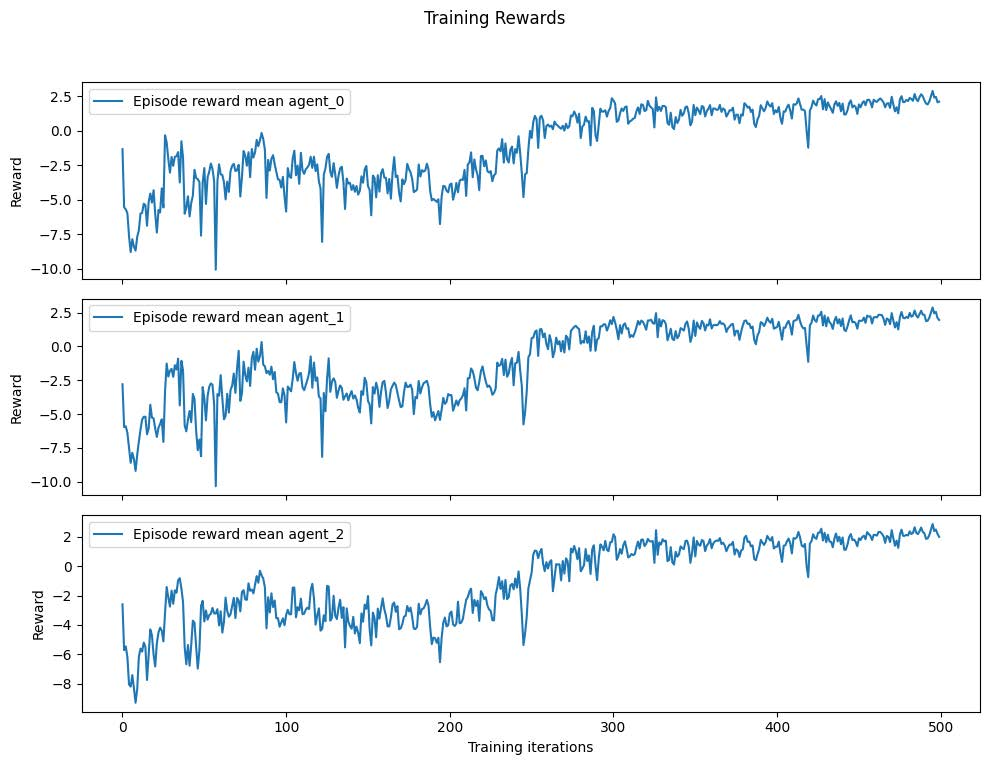
\includegraphics[width=0.75\linewidth]{figs/results.jpg}
    \caption{Agents performance after modifying a scalar hyper-parameter.}
    \label{fig:unstable_learning}
\end{figure}




}}


%%%%%%%%%%%%%%%%%%%%%%%%%%%%%%%%%%%%%%%%%%%%%%%%%

\newpage

{\fontfamily{lmss}\selectfont {\color{DarkBlue}

\begin{thebibliography}{9}

\bibitem{Freepik}
\href{https://www.freepik.com/free-vector/cute-artificial-intelligence-robot-isometric-icon_16717130.htm}{Cover image designed by freepik}

\bibitem{lowe2017multi}
Ryan Lowe, Yi I. Wu, Aviv Tamar, Jean Harb, Pieter Abbeel, and Igor Mordatch.
\newblock Multi-agent actor-critic for mixed cooperative-competitive environments.
\newblock In \emph{Advances in Neural Information Processing Systems (NeurIPS)}, 2017.
\newblock \href{https://arxiv.org/abs/1706.02275}{arXiv:1706.02275}


\end{thebibliography}


}}

%%%%%%%%%%%%%%%%%%%%%%%%%%%%%%%%%%%%%%%%%%%%%%%%%

\end{document}